
\documentclass{exam}

\usepackage{units} 
\usepackage{graphicx}
\usepackage[fleqn]{amsmath}
\usepackage{cancel}
\usepackage{float}
\usepackage{mdwlist}
\usepackage{booktabs}
\usepackage{cancel}
\usepackage{polynom}
\usepackage{caption}
\usepackage{fullpage}
\usepackage{xfrac}
\usepackage{enumerate}

\newcommand{\degree}{\ensuremath{^\circ}} 
\everymath{\displaystyle}

% \begin{figure}[H]
%   \centering
%   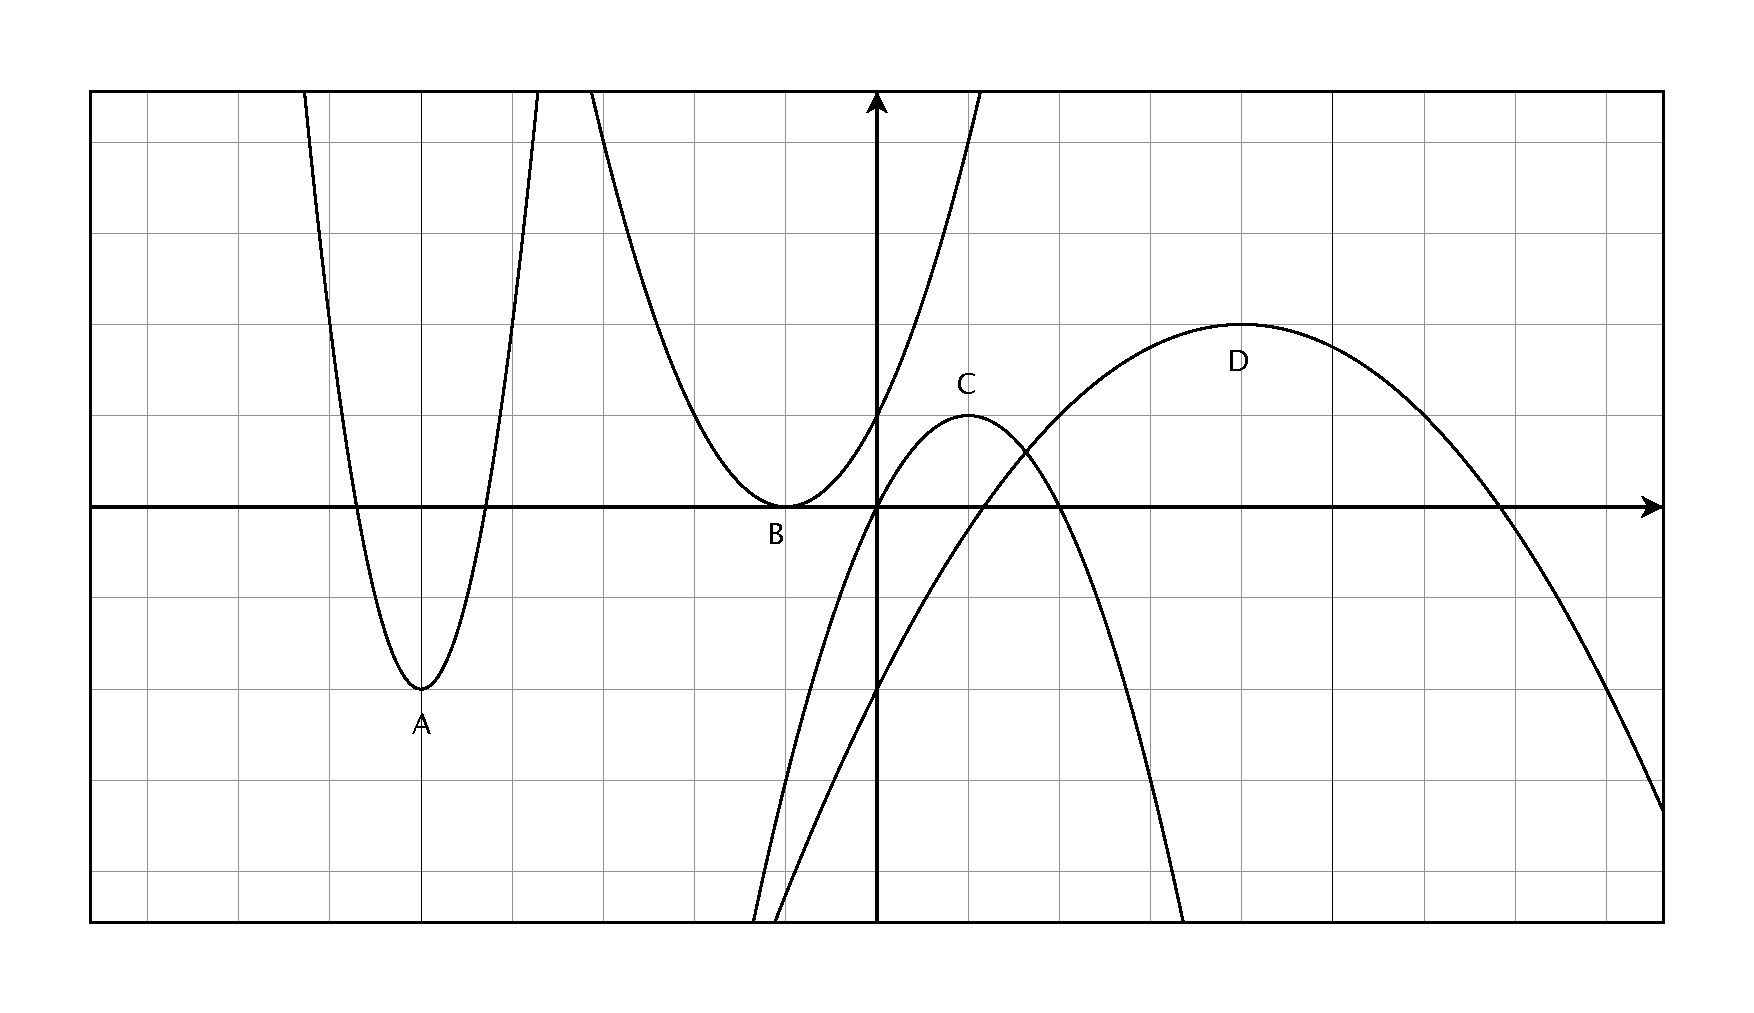
\includegraphics[scale=.3]{problem_7.eps}
%   \caption*{Problem 7}
% \end{figure}

% \begin{tabular}{cc}
% \toprule
% period & amplitude \\
% \midrule
%   $\pi$ & $2$ \\
% \bottomrule
% \end{tabular}

\printanswers

\ifprintanswers 
  \usepackage{2in1, lscape} 
\fi

\date{February 20, 2013}
\author{}
\title{Math 141 \\ Homework 6}

\begin{document}

\maketitle

\section{Schedule}
\begin{description*}
  \item[2/27] - Chapter 2 review
  \item[3/6] - Chapter 2 test
  \item[3/13 and 3/20] - Spring Break
\end{description*}

\section{Homework}

\begin{itemize*}
  \item Read Section 2.8
  \item Section 2.8: 1-25, 31-32, 35-36, 38, 41-44, 51-52, 65-68, 72, 74, 76, 78
\end{itemize*}

\section{Extra Credit}
Section 2.8, problems 81 

\ifprintanswers
  \pagebreak
  \begin{solution}
    \begin{description}

      \item[81]
        \begin{parts}
          \part The original equation can be described as ``multiply by two, add one, and divide by five.''  The inverse
          should be ``multiply by five, subtract one, and divide by two.''  This gives an inverse function of:
          \[
            f^{-1}(x) = \frac{5x - 1}{2}
          \]

          \part The original equation can be described as ``invert, negate, and add three.''  The inverse
          should be ``subtract three, negate, and invert''  This gives an inverse function of:
          \[
            f^{-1}(x) = \frac{1}{3 - x}
          \]

          \part The original equation can be described as ``cube, add two, and square root.''  The inverse
          should be ``square, subtract two, and cube root''  This gives an inverse function of:
          \[
            f^{-1}(x) = \sqrt[3]{x^2 - 2}
          \]

          \part The original equation can be described as ``multiply by two, subtract five, and cube.''  The inverse
          should be ``cube root, add five, and divide by two.''  This gives an inverse function of:
          \[
            f^{-1}(x) = \frac{\sqrt[3]{x} + 5}{2}
          \]

          \part
          This one is difficult because the first step requires two different operations on $x$: cube and multiple by two.

        \end{parts}

    \end{description}

  \end{solution}

  \pagebreak

  \section{Section 2.8}

  \begin{description}

    \item[1] not one-to-one
      
    \item[2] one-to-one
      
    \item[3] one-to-one
      
    \item[4] not one-to-one
      
    \item[5] not one-to-one
      
    \item[6] one-to-one
      
    \item[7] one-to-one

    \item[8] one-to-one

    \item[9] one-to-one
      
    \item[10] not one-to-one
      
    \item[11] This function is not one-to-one.  One way to show this is to find two $x$ values that both evaluate to
      zero:
      \begin{align*}
        x^2 - 2x &= 0 \\
        x(x - 2) &= 0 \\
        x &= \left\{ 0, 2 \right\} \\
      \end{align*}
      Since $f(0) = 0$ and $f(2) = 0$, the function is not one-to-one.
      
    \item[12] one-to-one

    \item[13] not one-to-one.  For example: $f(1) = f(-1) = 6$.  Any other positive/negative pair of x's would also work.

    \item[14] one-to-one since the domain is restricted to non-negative numbers.

    \item[15] not one-to-one.  For example: $f(1) = f(-1) = 1$.  Any other positive/negative pair of x's would also work.

    \item[16] one-to-one

\pagebreak

    \item[17] 
      \begin{parts}
        \part $f^{-1}(7) = 2$
        \part $f(-1) = 3$
      \end{parts}

    \item[18] 
      \begin{parts}
        \part $f^{-1}(18) = 5$
        \part $f(2) = 4$
      \end{parts}

    \item[19] 
      \begin{align*}
        5 - 2x &= 3 \\
        x      &= 1 \\
      \end{align*}
      Since $f(1) = 3$, $f^{-1}(3) = 1$

    \item[20] 
      \begin{align*}
        x^2 + 4x       &= 5 \\
        x^2 + 4x - 5   &= 0 \\
        (x - 1)(x + 5) &= 0 \\
        x              &= \{-5, 1\} \\
      \end{align*}
      Only 1 is in the domain of $f^{-1}(x)$, so $f^{-1}(5) = 1$.

    \item[21]
      \begin{align*}
        (f \circ g)(x) &= (x + 6) - 6 = x \\
        (g \circ f)(x) &= (x - 6) + 6 = x \\
      \end{align*}

    \item[22]
      \begin{align*}
        (f \circ g)(x) &= 3 \left( \frac{x}{3} \right) = x \\
        (g \circ f)(x) &= \frac{3x}{3} = x \\
      \end{align*}

    \item[23]
      \begin{align*}
        (f \circ g)(x) &= 2 \left( \frac{x + 5}{2} \right) - 5 = x \\
        (g \circ f)(x) &= \frac{(2x - 5) + 5}{2} = x \\
      \end{align*}

    \item[24]
      \begin{align*}
        (f \circ g)(x) &= \frac{3 - (3 - 4x)}{4} = x \\
        (g \circ f)(x) &= 3 - 4 \left( \frac{3 - x}{4} \right) = x \\
      \end{align*}

    \item[25]
      \begin{align*}
        (f \circ g)(x) &= \frac{1}{1/x} = x \\
        (g \circ f)(x) &= \frac{1}{1/x} = x \\
      \end{align*}

    \item[31]
      \begin{align*}
        y &= 2x + 1 \\
        x &= \frac{y - 1}{2} \\
        \\
        f^{-1}(x) &= \frac{x - 1}{2} \\
      \end{align*}

    \item[32]
      \begin{align*}
        y &= 6 - x \\
        x &= 6 - y \\
        \\
        f^{-1}(x) &= 6 - x \\
      \end{align*}

    \item[35]
      \begin{align*}
        y &= \frac{x}{2} \\
        x &= 2y \\
        \\
        f^{-1}(x) &= 2x \\
      \end{align*}

    \item[36]
      \begin{align*}
        y &= \frac{1}{x^2} \\
        x &= \frac{1}{\sqrt{y}} \\
        \\
        f^{-1}(x) &= \frac{1}{\sqrt{x}} \\
      \end{align*}

    \item[38]
      \begin{align*}
        y        &= \frac{x - 2}{x + 2} \\
        xy + 2y  &= x - 2 \\
        xy - x   &= -2y - 2 \\
        x(y - 1) &= -2y - 2 \\
        x        &= \frac{-2y - 2}{y - 1} \\
                 &= \frac{2y + 2}{1 - y} \\
        \\
        f^{-1}(x) &= \frac{2x + 2}{1 - x} \\
      \end{align*}

    \item[41]
      \begin{align*}
        y &= \sqrt{2 + 5x} \\
        y^2 &= 2 + 5x \\
        5x &= y^2 - 2 \\
        x &= \frac{y^2 - 2}{5} \\
        \\
        f^{-1}(x) &= \frac{x^2 - 2}{5} \\
      \end{align*}

    % do similar problem in class
    \item[42]
      \begin{align*}
        y &= x^2 + x \\
        x^2 + x + \frac{1}{4} &= y + \frac{1}{4} \\
        \left( x + \frac{1}{2} \right)^2 &= y + \frac{1}{4} \\
        x + \frac{1}{2} &= \sqrt{y + \frac{1}{4}} \\
        x &= - \frac{1}{2} + \sqrt{y + \frac{1}{4}} \\
        \\
        f^{-1}(x) &= - \frac{1}{2} + \sqrt{x + \frac{1}{4}} \\
          &= \frac{-1 + \sqrt{4x + 1}}{2} \\
      \end{align*}

    \item[43]
      \begin{align*}
        y   &= 4 - x^2 \\
        x^2 &= 4 - y \\
        x   &= \sqrt{4 - y} \\
        \\
        f^{-1}(x) &= \sqrt{4 - x} \\
      \end{align*}

    \item[44]
      \begin{align*}
        y   &= \sqrt{2x - 1} \\
        y^2 &= 2x - 1 \\
        x &= \frac{y^2 + 1}{2} \\
        \\
        f^{-1}(x) &= \frac{x^2 + 1}{2} \\
      \end{align*}

\pagebreak

    \item[51]
      \begin{align*}
        y &= 3x - 6 \\
        x &= \frac{y}{3} + 2 \\
        \\
        f^{-1}(x) &= \frac{x}{3} + 2 \\
      \end{align*}

      \begin{figure}[H]
        \centering
        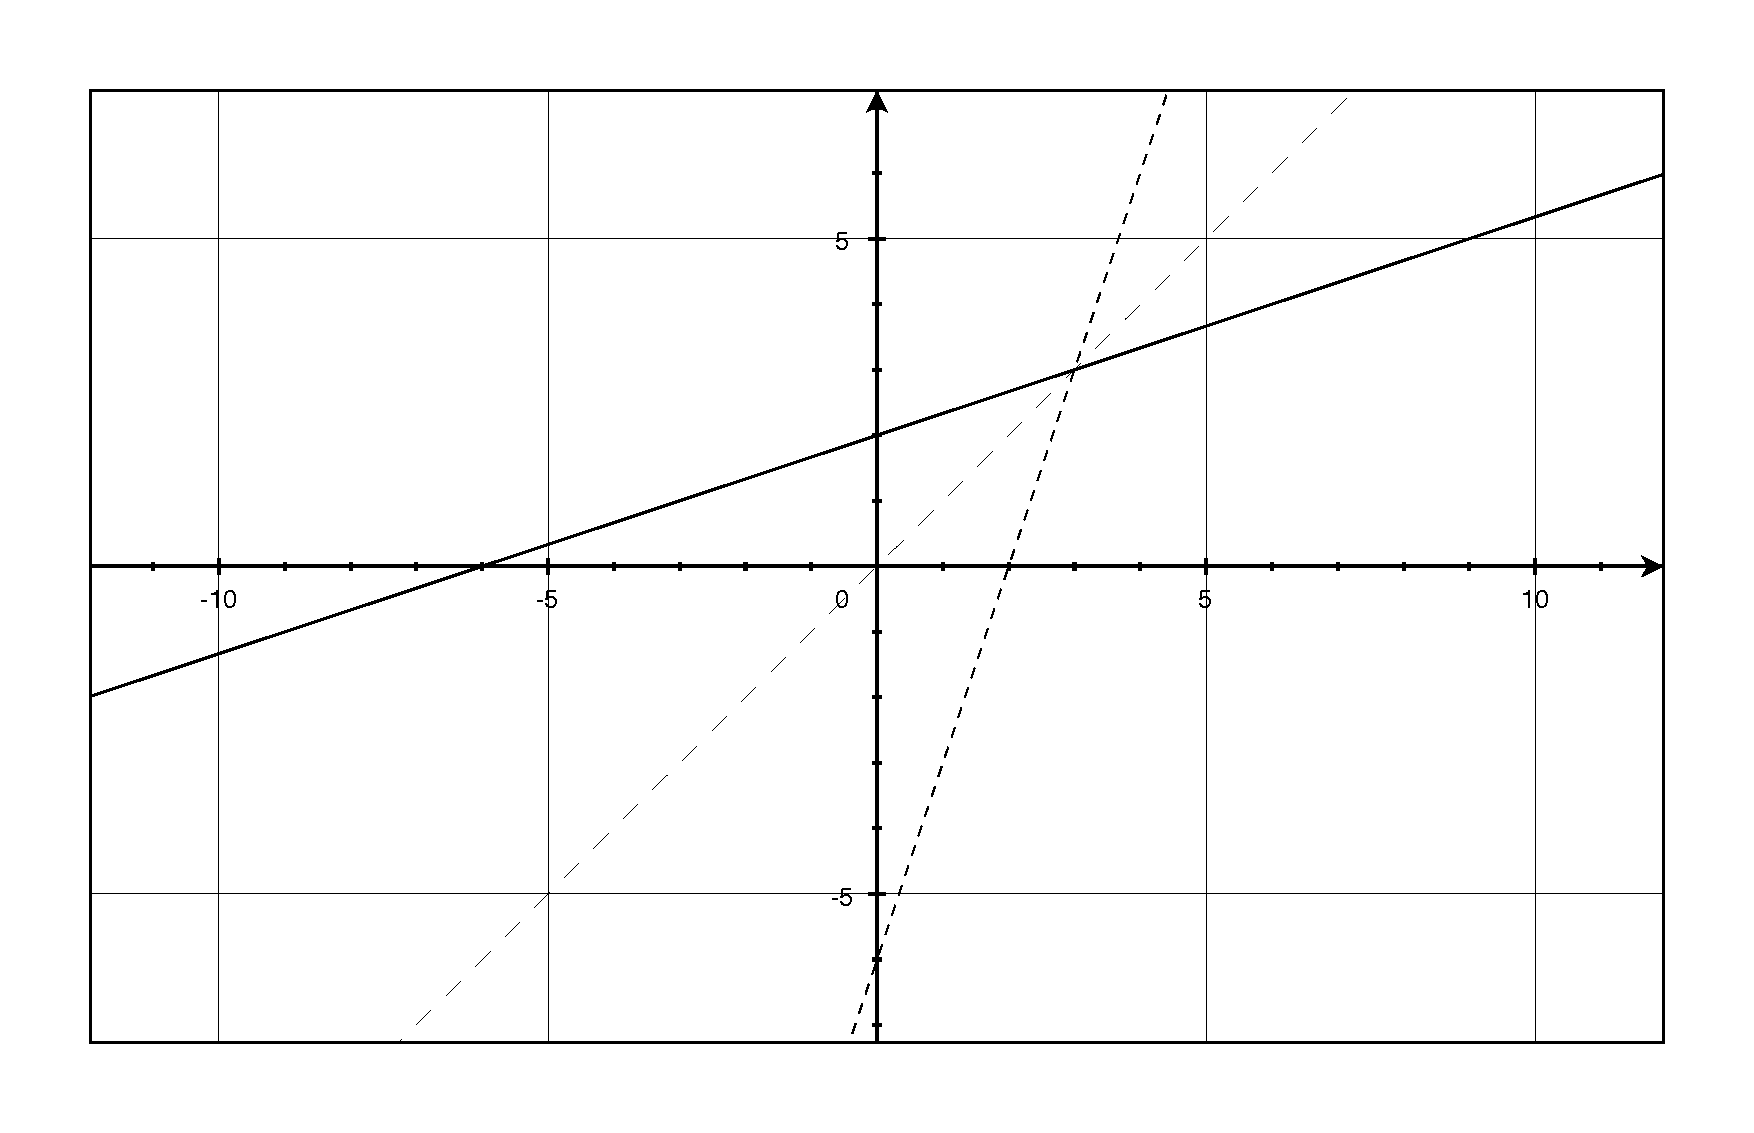
\includegraphics[scale=.3]{problem_51.eps}
        \caption*{Problem 51}
      \end{figure}
    
    \item[52]
      \begin{align*}
        y &= 16 - x^2 \\
        x &= \sqrt{16 - y} \\
        \\
        f^{-1}(x) &= \sqrt{16 - x} \\
      \end{align*}

      \begin{figure}[H]
        \centering
        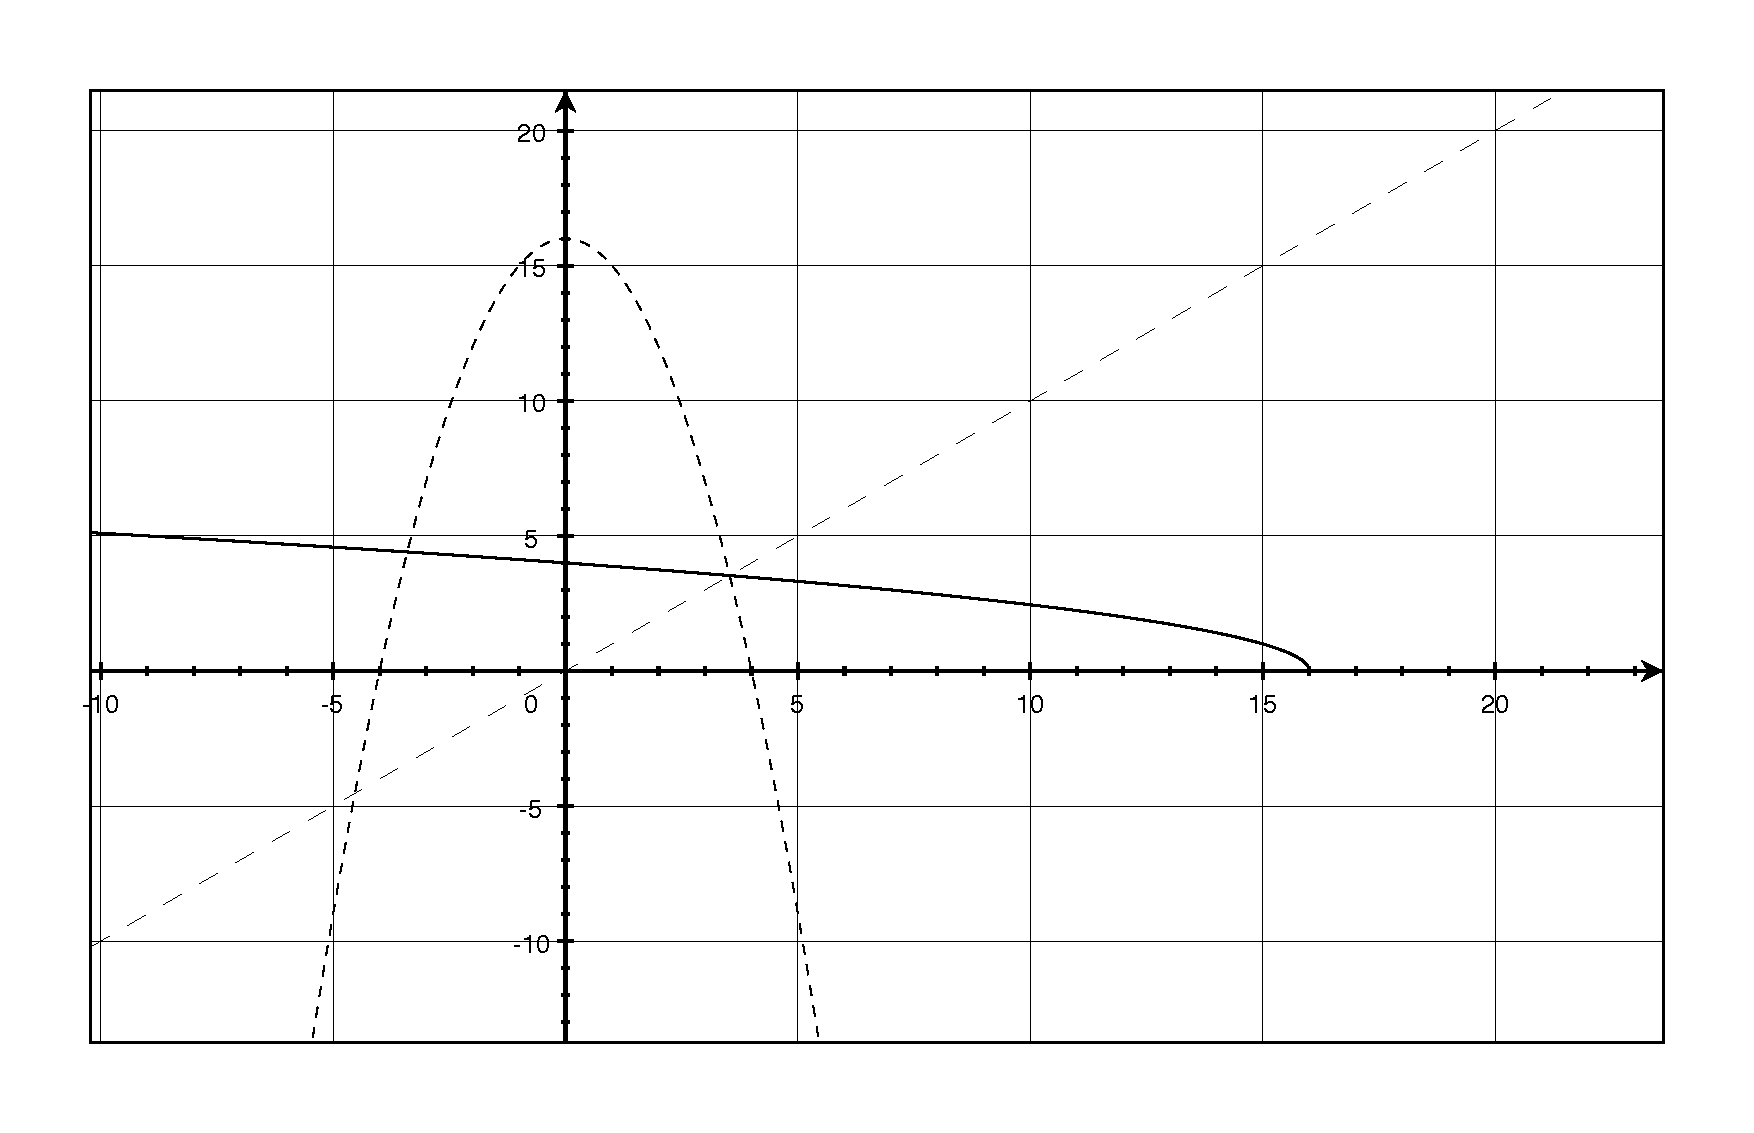
\includegraphics[scale=.3]{problem_52.eps}
        \caption*{Problem 52}
      \end{figure}
    
    \item[65]
      domain: $x \geq 0$
      \begin{align*}
        y &= 4 - x^2 \\
        x &= \sqrt{4 - y} \\
        \\
        f^{-1}(x) &= \sqrt{4 - x} \\
      \end{align*}

    \item[66]
      domain: $x \geq 1$
      \begin{align*}
        y &= (x - 1)^2 \\
        x &= \sqrt{y} + 1 \\
        \\
        f^{-1}(x) &= \sqrt{x} + 1 \\
      \end{align*}

    \item[67]
      domain: $x \geq -2$
      \begin{align*}
        y &= (x + 2)^2 \\
        x &= \sqrt{y} - 2 \\
        \\
        f^{-1}(x) &= \sqrt{x} - 2 \\
      \end{align*}

    \item[68]
      domain: $x \geq 3$
      If we restrict the domain in this way, the function is the same as $y = x - 3$, since the result is never
      negative.

      \begin{align*}
        y &= x - 3 \\
        x &= y + 3 \\
        \\
        f^{-1}(x) &= x + 3 \\
      \end{align*}

    \item[72]
      \begin{parts}
        \part
        \begin{align*}
          v                         &= 100 \left( 1 - \frac{t}{40} \right)^2 \\
          \frac{v}{100}             &= \left( 1 - \frac{t}{40} \right)^2 \\
          \frac{\sqrt{v}}{10}       &= 1 - \frac{t}{40} \\
          % \frac{\sqrt{v}}{10} - 1 &= -\frac{t}{40} \\
          t                         &= 40 - 4 \sqrt{v} \\
          \\
          V^{-1}(v) &= 40 - 4 \sqrt{v} \\
        \end{align*}

        \part
          $V^{-1}(v)$ is the time required to reach $v$ gallons of water remaining in the tank.  A better name for this
          function might be $T(v)$.

        \part
        $T(\unit[15]{gal}) = 40 - 4 \sqrt{15} \approx \unit[24.5]{minute}$.  
        
        It takes about 24.5 minutes for there to be 15 gallons of water remaining in the tank.
      \end{parts}
      
    \item[74]
      \begin{parts}
        \part
          \begin{align*}
            d &= -3p + 150 \\
            -3p &= d - 150 \\
            p &= 50 - \frac{d}{3} \\
            \\
            D^{-1}(x) &= 50 - \frac{d}{3} \\
          \end{align*}

          $D^{-1}(x)$ is the price you should charge if you want to sell $x$ units.  A better name for this function
          might be $P(x)$.

          \part $P(\unit[30]{units}) = \$40$.  If you have 30 units and want to sell them all, you should set the price
          at \$40.
      \end{parts}

    \item[76]
      \begin{parts}
        \part
          \[
            f(x) = 0.8159x
          \]
          If you have $x$ Canadian dollars, you can trade them in at the bank for $0.8159x$ US dollars.

        \part
          \[
            f^{-1}(x) = \frac{x}{0.8159} = 1.22564x 
          \]
          If you have $x$ US dollars, you can trade them in at the bank for $1.22564x$ Canadian dollars.
          
        \part
          \[
            f^{-1}(12,250) = 15,014.09
          \]
          12,250 US dollars can be exchanged for 15,014.09 Canadian Dollars.

      \end{parts}

    \item[78]
      \begin{parts}
        \part $f(x) = 0.85x$

        \part $g(x) = x - 1000$

        \part $H(x) = (f \circ g)(x) = 0.85(x - 1000) = 0.85x - 850$

        \part $H^{-1}(x) = \frac{x + 850}{0.85} = 1.17647x + 1,000.0$  This is the sticker price you would need, if you
          wanted to end up with a purchase price of $x$ dollars.

        \part $H^{-1}(13,000) = 16,294.11$.  This is the sticker price that would produce a purchase price of \$13,000
          after applying the rebate and discount.

      \end{parts}
  \end{description}
\else
  \vspace{8 cm}
  \begin{quote}
    {\em The degree of civilization in a society can be judged by entering its prisons. }
  \end{quote}

  \hspace{1 cm} --Fyodor Dostoevsky

  % Distrust all in whom the impulse to punish is powerful! (Nietzsche)

\fi

\end{document}

